%###############################################################
\section{Introduction}\label{sec:Intro}
%###############################################################

One of the exciting new directions of robotics is the design and development
of micro- and nanorobot systems, with the goal of letting a massive swarm of robots
perform complex operations in a complicated environment. Due to scaling 
issues, individual control of the involved robots becomes physically impossible:
while energy storage capacity drops with the third power of robot size,
medium resistance decreases much slower. As a consequence,
current micro- and nanorobot systems with many robots are steered and
directed by an external force that acts as a common control signal~\cite{Donald2013,Chiang2011,Hsi-Wen2012,Diller2013,Jing2013,Ou2013,Lanauze2013}.
These common control signals include global magnetic or electric fields,
chemical gradients, and turning a light source on and off.  

 \subsection{Selective Control with Global Inputs}
Clearly, having only one global signal that uniformly affects all robots at once
poses a strong restriction on the ability of the swarm to perform complex operations.
This control symmetry can be broken using interactions between the robot swarm
and obstacles in the environment. The key challenge is to establish
if interactions with obstacles are sufficient to perform complex operations, ideally by analyzing the complexity of possible logical operations.
 In previous work \cite{Becker2013f,Becker2014,Becker2014a},
we were able to demonstrate how a subset of logical functions can be implemented;
however, devising a fan-out gate (and thus the ability to replicate and copy information)
appeared to be prohibitively challenging. In this paper, we resolve this crucial question by
showing that only using unit-sized robots is insufficient for achieving computational
universality. Remarkably, adding a limited number of domino-shaped objects {\em is sufficient}
to let a common control signal, mobile particles, and unit-sized obstacles
simulate a computer. While this does not imply that large-scale computational 
tasks should be run on these particle computers instead of current electronic
devices, it establishes that future nano-scale systems are able to perform
arbitrarily complex operations {\em as part of the physical system}, instead
of having to go through external computational devices.


%\begin{figure}
 %  \centering
%\begin{overpic}[width =\columnwidth]{7tilefactory.jpg}
%\end{overpic}
%\caption{\label{fig:7tilefactory}A seven tile factory.  Each particle is actuated simultaneously by the same global control field.  The factory (black tiles) is designed so each clockwise control input assembles another component.
%}
%\end{figure}

\begin{figure}

\centering
\subfloat[]{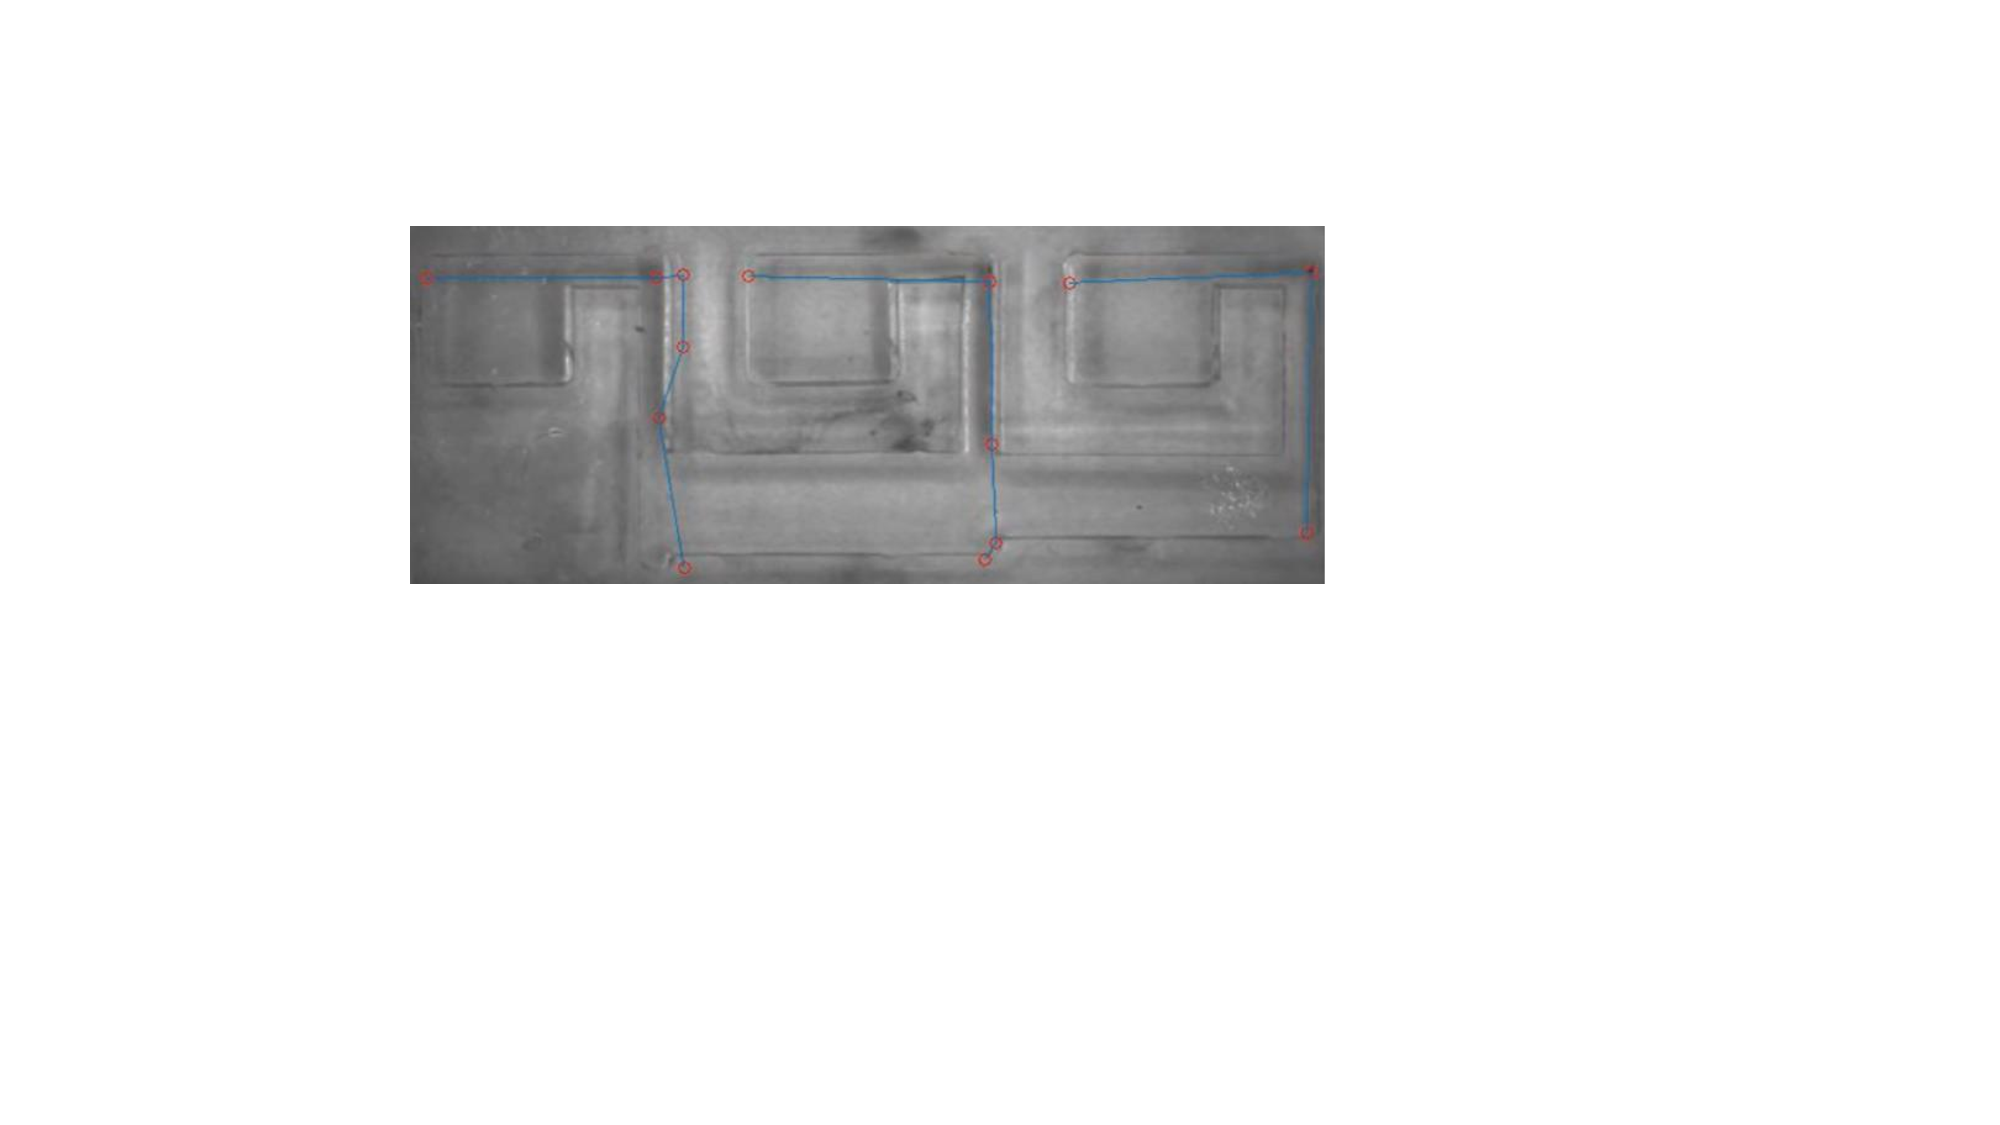
\includegraphics[width=3.1in]{fig1a.pdf}} 
\label{fig:fig1}
\newline
\subfloat[]{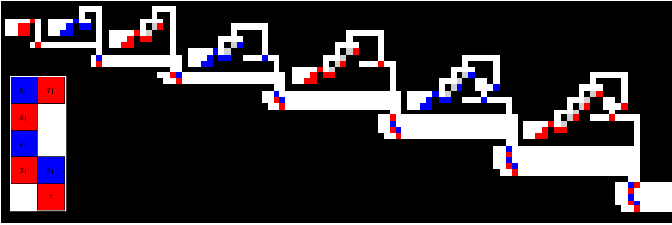
\includegraphics[width=3.1in]{fig1b1.pdf}}
\label{fig:fig2}
\caption{(a) A milli-scale magnetic based prototype.
 (b) A seven tile factory. Each particle is actuated simultaneously by the same global field. The factory is designed so each clockwise control input assembles another component.}
\label{fig:1} 

\end{figure}






%   \begin{figure}
%   \centering
%   \href{http://youtu.be/EJSv8ny31r8}{
%\begin{overpic}[width =\columnwidth]{DSC_0093lowres.JPG}%\put(30,-7){ $m=1$, partition 1}
%\end{overpic}}
%\caption{\label{fig:prototype}
%Gravity-fed hardware implementation of  particle computation.  The reconfigurable prototype is setup as a {\sc fan-out} gate using a 2$\times$1 robot (white). This paper proves that such a gate is impossible using only 1$\times$1 robots. \href{http://youtu.be/EJSv8ny31r8}{See the demonstrations in the video attachment \url{http://youtu.be/EJSv8ny31r8}.} }
%\vspace{-1em}
%\end{figure}

 \subsection{Model}\label{subsc:model}
  
This paper builds on the techniques for controlling many simple particles with uniform control inputs presented in \cite{Becker2013f,Becker2014,Becker2014a}, using the following rules:
\begin{enumerate}
\item A planar  grid \emph{workspace} $W$ is filled with a number of unit-square robots (each occupying one cell of the grid)  and some fixed unit-square blocks.  Each unit square in the workspace is either  \emph{free}, which a particle may occupy or \emph{obstacle} which a robot may not occupy.  Each square in the grid can be referenced by its Cartesian coordinates $\bm{x}=(x,y)$.
\item All particles are commanded in unison: the valid commands are  ``Go Up" ($u$), ``Go Right" ($r$), ``Go Down" ($d$), or ``Go Left" ($l$).  
\item Particles all move in the commanded direction until they 
	\begin{enumerate}
		\item hit an obstacle 
		\item hit a stationary particle. 
		\item share an edge with a compatible particle
	\end{enumerate}
	If a particle shares an edge with a compatible robot the two robots bond and from then on move as a unit.
A \emph{move sequence} $\bm{m}$ consists of an ordered sequence of moves $m_k$, where each $m_k\in\{u,d,r,l\}$  A representative move sequence is $\langle u,r,d,l,d,r,u,\ldots\rangle$. We assume the area of $W$ is finite and issue each command long enough for the robots to reach their maximum extent.
\end{enumerate}
